% Intended LaTeX compiler: xelatex
\documentclass[a4paper, 12pt]{article}
\usepackage{graphicx}
\usepackage{longtable}
\usepackage{wrapfig}
\usepackage{rotating}
\usepackage[normalem]{ulem}
\usepackage{amsmath}
\usepackage{amssymb}
\usepackage{capt-of}
\usepackage{hyperref}
\usepackage[danish]{babel}
\usepackage{mathtools}
\usepackage[margin=2.0cm]{geometry}
\hypersetup{colorlinks, linkcolor=black, urlcolor=blue}
\setlength{\parindent}{0em}
\parskip 1.5ex
\author{Matematik}
\date{Vibenshus Gymnasium}
\title{Vektorkanoner\\\medskip
\large Et lille spil med vektorer}
\hypersetup{
 pdfauthor={Matematik},
 pdftitle={Vektorkanoner},
 pdfkeywords={},
 pdfsubject={},
 pdfcreator={Emacs 28.1 (Org mode 9.5.5)}, 
 pdflang={Danish}}
\begin{document}

\maketitle
I dette spil skal I beskyde hinanden med jeres vektorkanoner. Spillet er en analog og simplificeret udgave af de klassiske spil \href{https://playclassic.games/games/strategy-dos-games-online/play-scorched-earth-online/}{Scorched Earth}, \href{https://playclassic.games/games/turn-based-strategy-dos-games-online/play-worms-online/}{Worms}, og nyere spil a la \href{http://www.shellshocklive.com/}{ShellShock live}.


\begin{center}
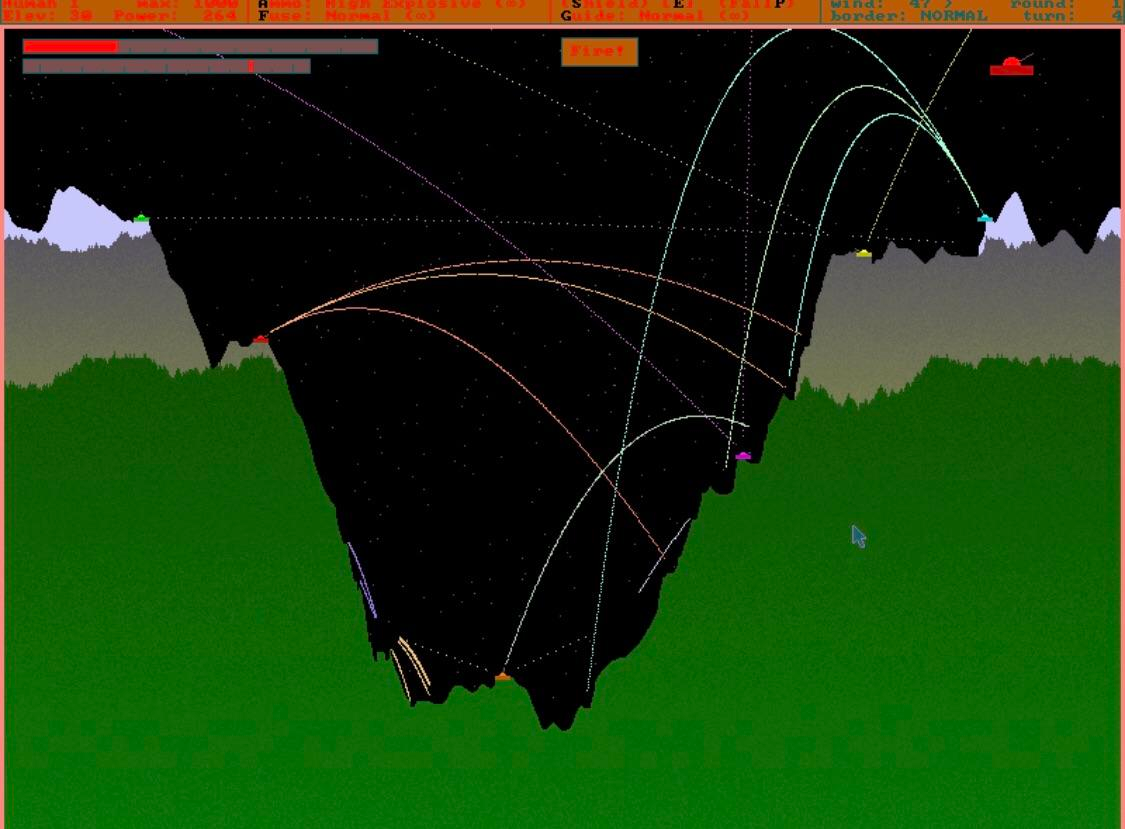
\includegraphics[height=3.5cm]{img/2022-10-26_13-46-35_screenshot.png}
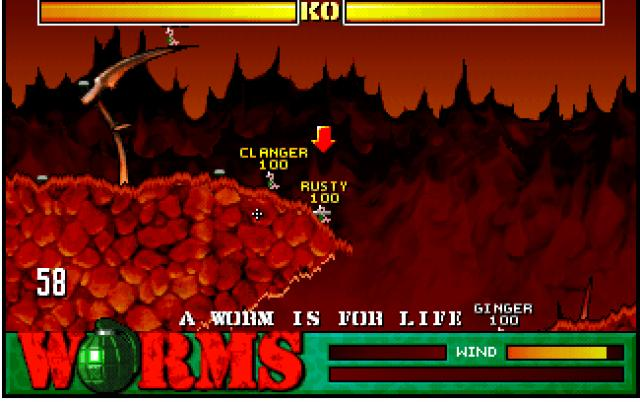
\includegraphics[height=3.5cm]{img/2022-10-26_13-54-06_screenshot.png}
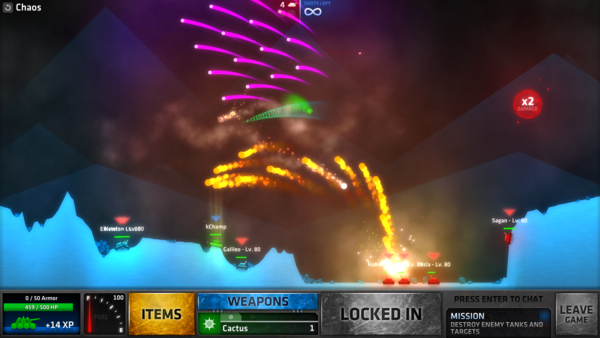
\includegraphics[height=3.5cm]{img/mindre.png}
\end{center}

Scorched Earth 1991, Worms 1995 og ShellShock live 2015.

I den simple version skal I forestille jer, at I har 3 kanoner hver, og det gælder om at ramme modstanderens kanoner.

\section*{Regler}
\label{sec:org3760467}
Reglerne er simple:

\begin{enumerate}
\item På et tegnet papir indtegner I et stort koordinatsystem med en eller begge akser langs papirets sider.
\item Hver spiller indtegner sine kanoner i hver ende af x-aksen. Kanonerne kan ikke stå oven i hinanden.
\item Træk lod om, hvem der skal starte.
\item Et skud foregår på følgende måde:
\begin{enumerate}
\item Kanonenskuglens starthastighedsvektor noteres. Denne kan ikke ændres, når et skud er i gang, og man kan ikke skyde vandret.
\item Udregn kanonkuglens nye hastighedsvektorer ved at holde x-koordinatet konstant og hele tiden trække 1 fra y-koordinatet.
\item Kanonkuglens bane tegnes ved at indtegne vektorerne i forlængelse af hinanden. Banen skulle gerne komme til at se ud som en parabel.
\item Hvis banen ender med at ramme en af modstanderens kanoner, har man fået en træffer, og modstanderens kanon er sat ud af spillet. Ellers har man ramt forbi, og må prøve igen i næste tur.
\end{enumerate}
\item Nu er det den anden spillers tur. Husk at skyde i den rigtige retning.
\item Man skiftes til at skyde, indtil den ene spiller har ramt alle modstanderens kanoner.
\end{enumerate}


\section*{Regneeksempel}
\label{sec:orgf568038}
Spilleren til venstre noterer starthastighedsvektoren \(\begin{pmatrix} 5 \\ 2 \end{pmatrix}\) på sit papir. De efterfølgende par vektorer vil så være \(\begin{pmatrix} 5 \\ 1 \end{pmatrix}\), \(\begin{pmatrix} 5 \\ 0 \end{pmatrix}\), \(\begin{pmatrix} 5 \\ -1 \end{pmatrix}\) og \(\begin{pmatrix} 5 \\ -2 \end{pmatrix}\).

På figuren kan eksemplet ses grafisk.

\begin{center}
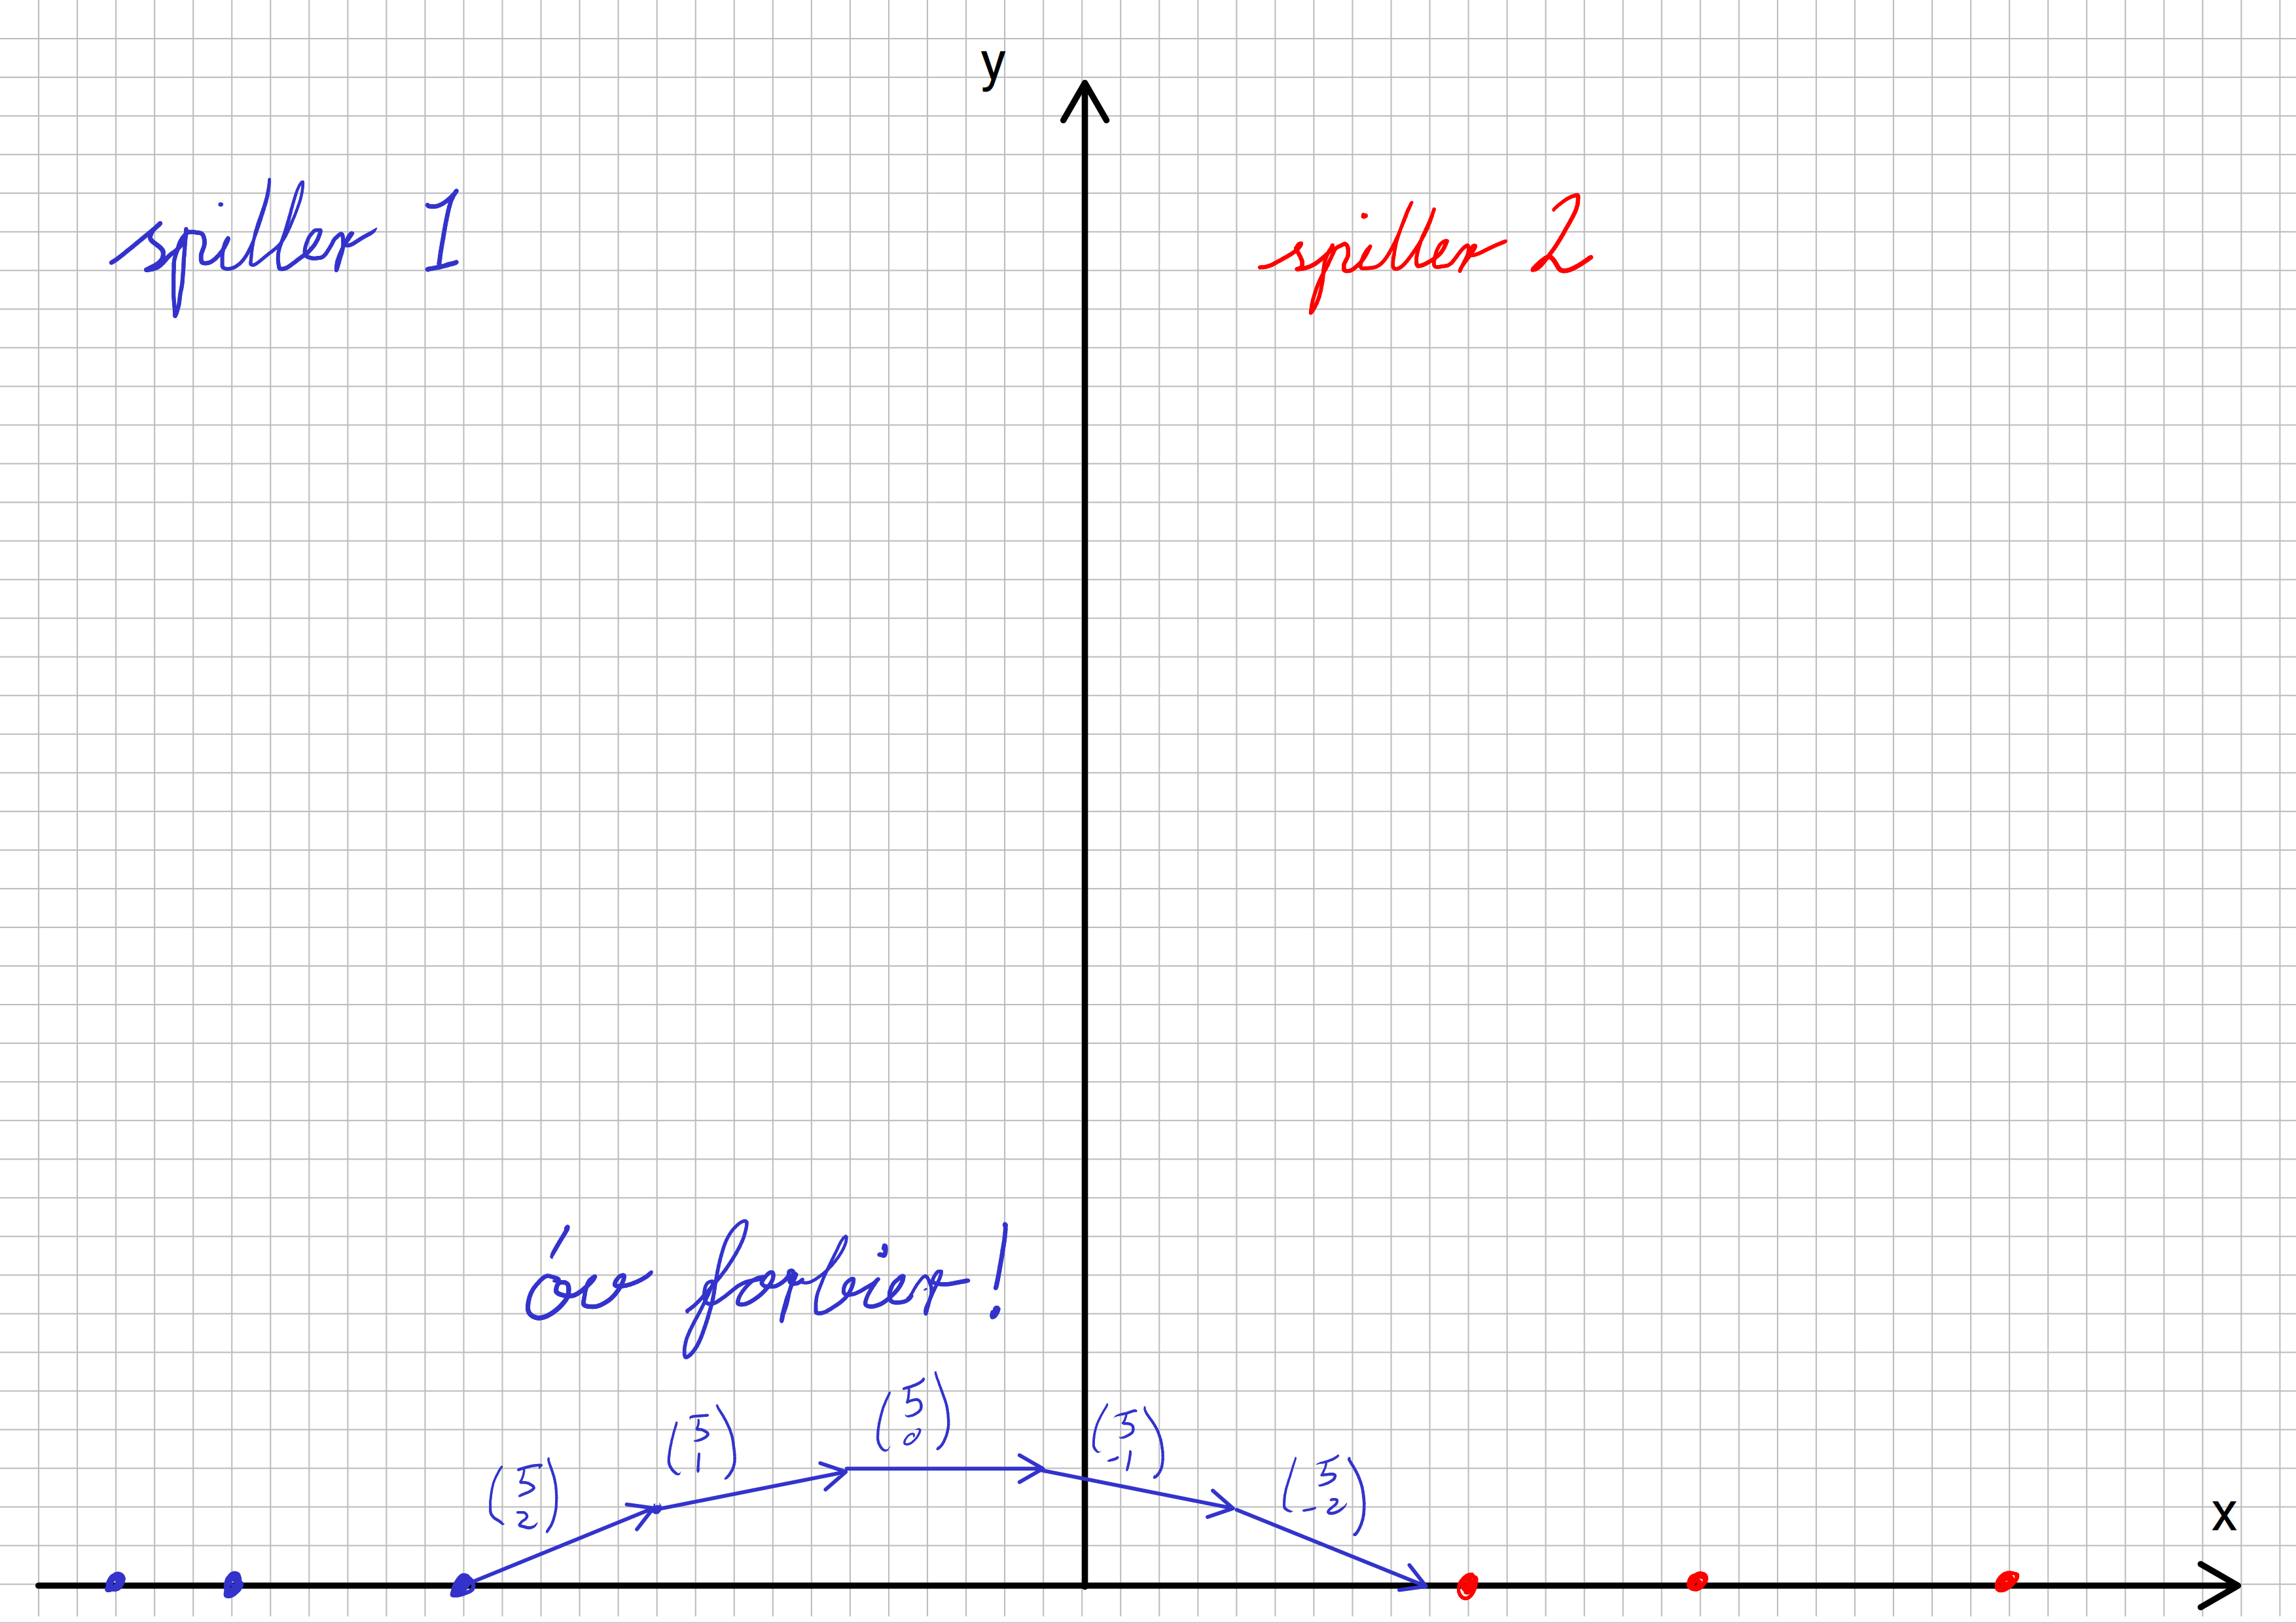
\includegraphics[width=.9\linewidth]{./img/Regneeksempel.png}
\end{center}

\newpage
\section*{Ekstra udfordringer}
\label{sec:orgb4c01bf}
Hvis det oprindelige spil bliver for nemt er her en række eksempler på tilføjelse, man kan anvende.

\begin{enumerate}
\item Man kan tegne et bakket landskab, og placere kanonerne på bakkerne og i dalene.
\item Man kan indsætte et højt bjerg eller lignende i midten af banen, som man skal skyde over.
\item Man kan spille med mod- og medvind.
x-koordinatet kan f.eks. vokse med 1 for hver vektor, når man har medvind, og falde med 1 for hver vektor i modvind.
\item Man kan spille på andre planeter, hvor tyngdekraften er større eller mindre (Der skal mere eller mindre end 1 fra på y-aksen hver gang).
\item Man kan begrænse kanonernes skudkraft ved at sætte en grænse for, hvor lang starthastighedsvektoren må være.
\item Man kan indsætte infanterienheder, som rykker 1 felt frem for hver tur. Hvis infanteriet når frem til en spillers kanon er den sat ud af spillet. Man skal derfor også få skudt infanteriet ned.
\end{enumerate}

Det er altså kun fantasien, som sætter grænser.

God spillelyst.
\end{document}